\chapter{Implementación}
En este capítulo vamos a pasar a explicar con 
total detalle cada uno de los algoritmos implementados.
Explicaremos tanto sus fundamentos, como su motivación
y por último la implementación que se ha llevado a cabo.

\section{LOF}
Para el desarrollo y implementación de este algoritmos se 
ha utilizado como referencia tanto el libro \cite{aggarwalOutlierAnalysis2017}
como el artículo donde se presenta el algoritmo \cite{breunigLOFIdentifyingDensitybased2000}.


Local Outlier Factor (LOF), o en español factor de 
valor atípico local, es una cuantificación 
del valor atípico de un punto perteneciente al conjunto de datos.
Esta cuantificación es capaz de ajustar las variaciones
en las densidades locales. De modo que el objetivo será obtener 
una puntuación a través del análisis de densidad local a cada punto.
Para el cálculo de dicha puntuación vamos a desarrollar varias 
definiciones necesarias para comprender el desarrollo


En primer lugar, para un dado punto $\overline{X}$,
definimos $D^k(\overline{X})$ como la distancia del 
k-vecino más cercano de $\overline{X}$. Normalmente
el conjunto de puntos que se encuentran a una distancia
$D^k(\overline{X})$ de  $\overline{X}$ contiene k puntos.
Esto no es estrictamente necesario ya que podemos tener puntos
a la misma distancia exacta y por tanto tener más de k
puntos.


Ahora podemos definir la reachability distance o distancia de
alcance en español, del punto  $\overline{X}$ con respecto
del punto  $\overline{Y}$: 

\begin{center}
    $R_k(\overline{X},\overline{Y}) = max ( dist(\overline{X},\overline{Y}), D^k(\overline{X}) ) $
\end{center}

La distancia de alcance, como podemos imaginar no es simétrica
entre $\overline{X}$ y $\overline{Y}$ ya que el k-vecino más cercano
de  $\overline{Y}$ puede ser otro totalmente distinto al de 
$\overline{X}$. Cuando $\overline{Y}$ está en una región densa y la
distancia entre $\overline{X}$ y $\overline{Y}$ es amplia, la distancia
de alcance de $\overline{X}$ usará la distancia entre ambos puntos $dist(\overline{X},\overline{Y})$. 
Por otro lado, cuando la distancia entre ambos puntos sea pequeña, la distancia de
alcance se suaviza con la distancia al k-vecino más cercano. Cuanto mayor
sea el valor de k mayor será el suavizado aplicado.


El cálculo de esta distancia se hace visible en la siguiente figura 
del artículo  \cite{breunigLOFIdentifyingDensitybased2000}: 

\begin{figure}[h]
    \center{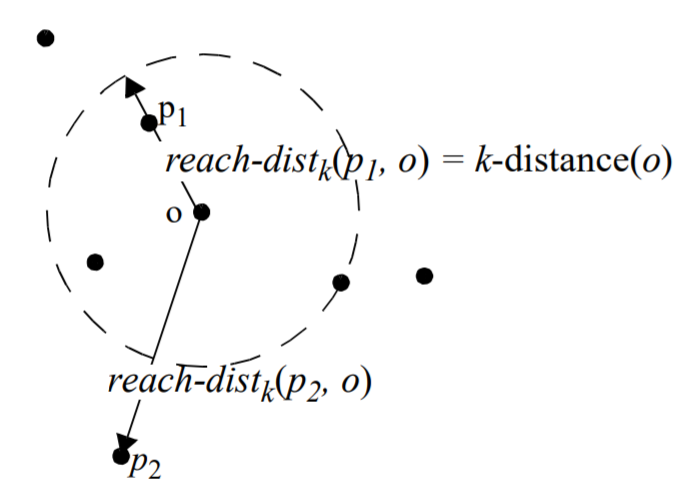
\includegraphics[width=\textwidth]
    {imagenes/distancia-alcance.png}}
    \caption{\label{fig:base-abstraccion} Abstracción de la clase general sklearn}
\end{figure}

Ahora podemos definir la media de la distancia de alcance $AR_k$, teniendo
en cuenta que el conjunto $L_k(\overline{X})$ es el conjunto de puntos a una
distancia menor que el k-vecino más cercano. 

\begin{center}
    $AR_k(\overline{X}) = MEDIA_{\overline{Y} \in L_k(\overline{X}) } R_k(\overline{X},\overline{Y})$
\end{center}

Aquí la media representa la media de valores de un conjunto de valores.
Con esta definición podemos definir el valor LOF


\begin{center}
    $LOF_k(\overline{X}) = AR_k(\overline{X}) \cdot MEDIA_{\overline{Y} \in L_k(\overline{X}) }       \frac{1}{AR_k(\overline{Y})} $
\end{center}

El uso de relaciones de distancia en la definición asegura que el
comportamiento de la distancia local se tenga en cuenta en esta definición.
Como resultado, los valores LOF para los objetos en un clúster
a menudo son cercanos a 1, cuando los puntos de datos en el clúster
se distribuyen de manera homogénea. Por ejemplo, en el caso de la 
figura \ref{fig:densidad}, los valores de LOF de los puntos de datos
en ambos grupos serán cercanos a 1, aunque las densidades de los dos 
grupos sean diferentes.

El cálculo de LOF puede ser visto como una normalización de la distancia
de alcance de un punto, donde el factor de normalización usado es la 
media armónica. Ambos casos son en principio válidos, aunque nosotros usaremos
la primera definición por simplicidad e interpretación.


Por otro lado, cabe mencionar que LOF también puede considerarse como
un algoritmo basado en distancias relativamente con suavizado. Se calculan
las distancias entre puntos para el cálculo de la distancia de alcance.
Como ya mencionábamos podemos dar ciertos enfoques ya que usan conceptos
de los tres tipos de algoritmos que comentábamos en el capitulo 
\ref{cap:Analisis}.

Aquí tenemos el pseudocódigo del algoritmo LOF. En nuestro caso implementado
en Python y haciendo el máximo uso posible de estructuras de datos eficientes,
para conseguir una implementación veloz y eficiente.

\begin{codigo}
    \begin{algorithmic}[1]
    \Function {LOF}{Matrix de datos D, k}
    \State \parbox[t]{305pt}{distancias = calcular matrix de distancias con k-nn}
    \ForEach{$x_i \in \mathcal D $}
    \State \parbox[t]{305pt}{ $AR_k(x_i) = MEDIA_{y \in L_k(x_i) } R_k(x_i,y)$}
    \State {$LOF_k(x_i) = AR_k(x_i) \cdot MEDIA_{y \in L_k(x_i) }       \frac{1}{AR_k(y)} $}
    \EndFor 
    \State \Return Puntuaciones: $LOF_k$
    \EndFunction 
    \end{algorithmic}
\end{codigo}


\section{LOOP}
Esta técnica combina varios conceptos. en primer lugar, la idea de localidad,
los algoritmos basados en densidad como LOF. Por otro lado, LOCI con conceptos
probabilísticos para modelar la puntuación de una anomalía. Un enfoque probabilístico 
significa ofrecer una tolerancia natural a los efectos de ruido en los datos. 
Los enfoques tradicionales como LOF y LOCI pueden incluso enfatizar tales efectos. 
Por ejemplo, LOF se basa en comparar las k distancias de los puntos, es decir, 
las distancias de los puntos a su k-vecino más cercano. Una elección inapropiada 
(localmente) de k puede causar resultados malos como ya comentamos anteriormente.

En esta técnica se propone una puntuación que incluye una normalización para 
convertir en independiente de la distribución de datos específica en un conjunto 
de datos dado, así como una motivación estadísticamente sólida para obtener valores 
en el rango de [0, 1], fácilmente interpretable como la probabilidad de un 
determinado punto en ser una anomalía.

Vamos a explicar detalladamente este nuevo enfoque el cual podemos encontrar con 
más detalle en el artículo de referencia \cite{kriegelLoOPLocalOutlier2009}. 
Seguiremos la misma notación del artículo para conseguir una comprensión 
más fácil.

Asumimos como $D$ el conjunto de datos con $n$ puntos o objetos y $d$ dimensiones.
Ahora definimos el concepto de distancia probabilística de un objeto $ o \in D$ 
en un contexto de $S \subseteq D$ y a la cual nos referimos como $pdist(o,S)$. 
Esta distancia se define como:

\[ 	\forall s \in S: P[d(o,s) \leq pdist(o,S)] \geq \varphi  \]

Intuitivamente, estamos cogiendo una esfera alrededor de $o$ con radio $pdist $
cubre cualquier elemento en el conjunto de contexto $S$ con una probabilidad de
$\varphi$. La distancia probabilística $pdist (o, S)$ de $o$ a $S$ se puede 
interpretar como la extensión estadística del conjunto de contexto S. La principal 
diferencia con la extensión (normal) de un conjunto de puntos es que la extensión 
estadística permite deliberadamente algún error. El recíproco de la distancia 
probabilística puede verse como una estimación de la densidad:

\[ 	pdens(S) = \frac{1}{pdist(o,S)} \]

Podemos simular la noción estadística clásica y sólida de valores atípicos
definidos como objetos que se desvían más de un $\lambda$ dado la desviación
estándar $\sigma$ de la media. Para ello usamos la siguiente difinición de $\lambda$

\[ 	 \lambda = \sqrt{2} \cdot erf^{-1}(\varphi) \]

Donde $erf$ representa la función de error Gaussiana. Esto nos permite determinar
nuestro error a través de los diferentes valores de $\lambda$.


Asumiendo que o se encuentra en el centro de $S$ podemos calcular la desviación 
estándar como:

\[ \sigma(o,S) = \sqrt{ \frac{\Sigma_{s \in S} d(o,s)^2 }{|S|} }    \]

Con estas consideraciones podemos redefinir la distancia probabilística con
la siguiente expresión:


\[ pdist(\lambda,o,S) := \lambda \cdot \sigma(o,S) \]

Intuitivamente, esta distancia de conjunto probabilístico estima la densidad 
alrededor de $o$ en función de $S$. El parámetro $\lambda$ da control sobre 
la aproximación de la densidad. Sin embargo, es solo un factor de normalización 
que solo afecta el contraste en las puntuaciones resultantes. La clasificación 
de los valores atípicos no se verá afectada por $\lambda$.

Para el correcto funcionamiento de esta técnica debemos realizar varias suposiciones.
La más importante es que estamos suponiendo que el conjunto $S$ esta centrado $o$.
Esta suposición no es fácil de conseguir ya que estamos conformando el conjunto $S$
como una distancia radio. Esto nos da ciertas ventajas y es que la técnica combina
la ventaja de dos mundos, los enfoques basados en densidad que no asumen 
ninguna distribución de datos específica y los conceptos matemáticos 
sólidos de los métodos estadísticos. Con estas razones y teniendo en cuenta que 
$E[  \; ]$ se refiere a la media definimos el factor local de anomalía o LOF probabilístico:

\[ PLOF_{\lambda,S}(o) := \frac{pdist(\lambda,o,S(o))}{E_{s \in S(o)} [pdist(\lambda,s,S(s))]} -1 \] 


El valor $PLOF$ de un objeto $o \in D$ calcula la relación de la 
estimación para la densidad alrededor de $o$ que se basa en $S(o)$ 
y el valor esperado de las estimaciones para las densidades alrededor 
de todos los objetos en el conjunto de contexto $S(o)$
Debemos de resaltar que a pesar de obtener valores parecidos a los de LOF,
estos no son aun probabilidades ni están normalizados.

Para lograr una normalización que haga que la escala de PLOF sea 
independiente de la distribución de datos en particular, el valor 
agregado nPLOF se obtiene con la siguiente expresión:

\[ nPLOF := \lambda \cdot \sqrt{E[PLOF^2]}\]

Este valor puede verse como un tipo de desviación estándar de
valores PLOF.

Ahora aplicamos la Función de Error Gaussiana (erf) para obtener 
un valor de probabilidad, el \textbf{Local Outlier Probability (LoOP)}

\[ LoOP(o) := max ( 0, erf( \frac{PLOF_{\lambda,S}(o)}{nPLOF \cdot \sqrt{2}})    )\]


El valor de LoOP estará cerca de 0 para puntos dentro de regiones densas 
y cerca de 1 para valores atípicos basados en densidad local.
En otras palabras, si bien una puntuación de valores atípicos de $x$ 
calculada por un enfoque local como LOF designará diferentes grados 
de valores atípicos para diferentes regiones del mismo conjunto de 
datos y no se puede comparar con una puntuación de $x$ en un conjunto 
de datos diferente, los valores de LoOP son consistentes sobre el
conjunto completo de datos y en múltiples conjuntos de datos. El resultado
es una probabilidad de ser anomalía en el intervalo [0-1], por lo que 
podemos comparar entre cualquier conjunto de datos.
Esto nos aporta una mejor interpretabilidad de los resultados frente a otros
métodos.

Vamos ahora a exponer el pseudocódigo de este algoritmo y el usado para su
implementación en nuestra biblioteca. En primer lugar, debemos comentar que
hemos usado el algoritmo k-nn como base para construir los conjuntos S,
asegurando de este modo que nuestro objeto o sea el centro del volumen.

\begin{codigo}
    \begin{algorithmic}[1]
    \Function {LOOP}{Matrix de datos D, k, $\lambda$ }
    \State \parbox[t]{305pt}{calcular matrix de distancias con k-nn y conjunto $S(o)$}
    \ForEach{$o \in \mathcal D $}
    \State \parbox[t]{305pt}{ $ \sigma(o,S) = \sqrt{ \frac{\Sigma_{s \in S} d(o,s)^2 }{|S|} } $}
    \State {$pdist(\lambda,o,S) := \lambda \cdot \sigma(o,S) $}
    \State {$PLOF_{\lambda,S}(o) := \frac{pdist(\lambda,o,S(o))}{E_{s \in S(o)} [pdist(\lambda,s,S(s))]} -1 $}
    \State {$nPLOF := \lambda \cdot \sqrt{E[PLOF^2]} $}
    \State {$LoOP(o) := max ( 0, erf( \frac{PLOF_{\lambda,S}(o)}{nPLOF \cdot \sqrt{2}})    ) $}
    \EndFor
    \State \Return Puntuaciones: $LOOP$
    \EndFunction 
    \end{algorithmic}
\end{codigo}

En nuestro caso al realizar una implementación en Python hemos usado la comprensión
de listas en lugar de un bucle for y de este modo conseguimos una mayor velocidad.
Con esto conseguimos que el algoritmo sea realmente útil reduciendo su tiempo
de computación.


\section{LDOF}
Esta técnica busca resolver el problema de la detección de anomalías cuando los 
datos que queremos analizar son dispersos. Muchas técnicas suponen que los datos
se agrupan en unos pocos grupos, pero en los datos reales existen multitud de conjuntos
de datos donde los puntos se presentan dispersos.


Local Distance-based Outlier Factor (LDOF) o Factor de Factor de valores atípicos 
basados en la distancia local en español, es sensible a los valores atípicos en 
conjuntos de datos dispersos. LDOF utiliza la distancia relativa de un 
objeto a sus vecinos para medir la cantidad de objetos que se desvían de 
su vecindario disperso. Cuanto más alto es el grado de violación que 
tiene un objeto, más probable es que el objeto sea un valor atípico. 
Para simplificar la configuración de parámetros en aplicaciones del mundo
real, la técnica top-n se emplea en este enfoque.

Como referencia para el desarrollo de este algoritmo 
se ha usado el artículo donde los autores los presentan \cite{zhangNewLocalDistancebased2009}

La motivación de este algoritmo nace de la ineficiencia de algoritmos como
k-nn o LOF en datos dispersos. Para ver este hecho vamos a mostrar un ejemplo
donde esto se hace visible. Usamos el ejemplo que plantean los autores:

\begin{figure}[h]
    \center{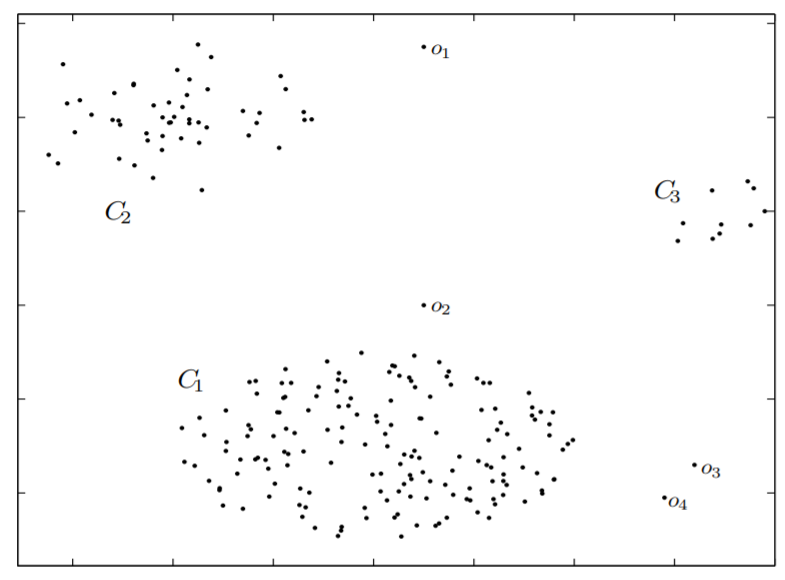
\includegraphics[width=\textwidth]
    {imagenes/datos-dispersos.png}}
    \caption{\label{fig:datos-dispersos} Ejemplo de datos dispersos}
\end{figure}

Analizamos el comportamiento de k-nn, cuando k es mayor 
que la cardinalidad de C3 (10 en este caso), algunos objetos en C1 se 
convierten en vecinos de los objetos en C3. Por lo tanto, la distancia 
del objeto puede ser mayor que los valores atípicos.
En el caso de LOF, ya que la densidad de C3 es más pequeña que la de C1,
la clasificación de o1, o2, o3 y o4$o_1, o_2, o_3, o_4$ 
como valores atípicos se complica y puede ser errónea.
Por tanto, en nuestro enfoque la idea principal será medir cómo 
un objeto se desvía de su sistema de vecindad como un factor de valor 
atípico.


Ahora vamos a explicar las definiciones y cálculos necesarios para la obtención
final de la puntuación. Para mantener la coherencia con el artículo de referencia
mantendremos la misma anotación. Definimos $N_p$ como el conjunto de los k-vecinos
más cercanos del punto $x_p$, excluyéndolo del propio conjunto. Definimos
la distancia de k-vecinos más cercanos como:


\[ \bar{d}_{x_p}  := \frac{1}{k} \sum_{x_i \in N_p} dist(x_i,X_p)\]

Ahora definimos la distancia interna de $x_p$ como la distancia promedio 
entre los objetos en $N_p$

\[     \bar{D}_{x_p}  := \frac{1}{k(k-1)}  \sum_{x_i,x_i'  \in  N_p i \neq i' }   \]


Finalmente se define el factor de valor atípico basado en la distancia local 
(LDOF)de $x_p$ como:
\[    LDOF_k(x_p) := \frac{\bar{d}_{x_p}}{\bar{D}_{x_p}}       \]

\begin{figure}[h]
    \center{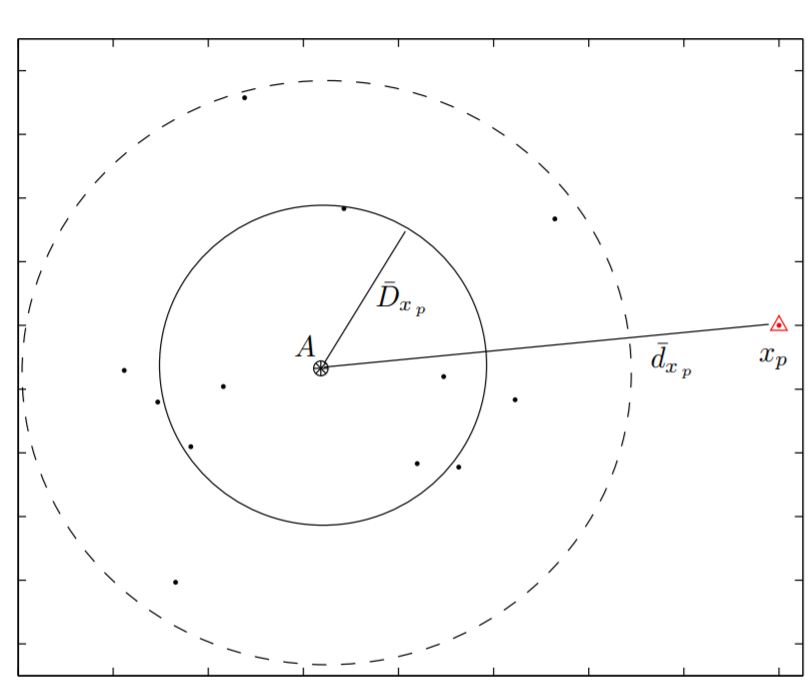
\includegraphics[width=\textwidth]
    {imagenes/LDOF.png}}
    \caption{\label{fig:LDOF} Ejemplo de funcionamiento de LDOF}
\end{figure}

La definición de LDOF, como se muestra en la Figura \ref{fig:LDOF}, 
claramente considera que $x_p$ está fuera de su región de vecindario. 
El valor LDOF de $x_p$ es obviamente mayor que 1, lo que indica que $x_p$
es un valor atípico. A través de este ejemplo, podemos ver que LDOF 
puede capturar efectivamente la condición de anomalía de un objeto 
entre un vecindario disperso. Además, a medida que k crece, LDOF 
toma más objetos en consideración y la vista de LDOF se vuelve cada 
vez más global. Si un objeto está lejos de su gran sistema de vecindad, llevado al 
extremo todo el conjunto de datos, es definitivamente un valor 
atípico. Por lo tanto, la precisión de detección del método podría ser
estable en un amplio rango de k.

\begin{codigo}
    \begin{algorithmic}[1]
    \Function {LDOF}{Matrix de datos D, k }
    \State \parbox[t]{305pt}{calcular matrix de distancias con k-nn}
    \ForEach{$X_p \in \mathcal D $}
    \State \parbox[t]{305pt}{ $ \bar{d}_{x_p}  := \frac{1}{k} \sum_{x_i \in N_p} dist(x_i,X_p) $}
    \State {$\bar{D}_{x_p}  := \frac{1}{k(k-1)}  \sum_{x_i,x_i'  \in  N_p i \neq i' }$}
    \State {$PLOF_{\lambda,S}(o) := \frac{pdist(\lambda,o,S(o))}{E_{s \in S(o)} [pdist(\lambda,s,S(s))]} -1 $}   
    \State {$ LDOF_k(x_p) := \frac{\bar{d}_{x_p}}{\bar{D}_{x_p}} $}
    \EndFor
    \State \Return Puntuaciones: $LDOF_k$
    \EndFunction 
    \end{algorithmic}
\end{codigo}

Este es el pseudocódigo usado para la implementación en nuestra biblioteca.
Al igual que pasaba con LDOF el bucle queda eliminado con el uso de la 
comprensión de listas de Python por motivos de eficiencia.


\section{PINN-LOF}
Esta técnica nace a partir de la idea de que existen áreas de 
aplicación en las que se encuentran con frecuencia problemas de 
rendimiento debido al gran tamaño de los conjuntos de datos y las 
dimensiones incluyen texto y datos médicos, para los cuales aún no 
se han investigado adecuadamente los beneficios potenciales del 
análisis de valores atípicos locales. En general, las dificultades 
de escalabilidad inherentes generalmente impiden el uso de técnicas 
de valores atípicos locales estándar para obtener resultados útiles 
en conjuntos de datos tan grandes y de gran dimensión. Esta técnica
se presenta en el siguiente artículo \cite{vriesFindingLocalAnomalies2010}

El mayor desafío es cómo lidiar con la 'maldición de la dimensión:
a medida que la dimensión de los datos crece, las medidas de 
distancia pierden su capacidad discriminativa, y las técnicas de 
indexación convencional ya no son efectivas para administrar la 
búsqueda de vecinos requerida por los métodos basados en distancias y 
densidad.


Existen varias técnicas para intentar mitigar estos problemas como el uso
de estrategias de sampling o métodos de indexación con poda. Aunque estas
quedan muy limitadas a casos específicos.

En este algoritmo se propone un método de detección de valores 
atípicos locales proyectivo basado en LOF, al que llamamos Vecino 
Más Cercano Indexado por Proyección, Más conocido por su nombre en
ingles Projection-Indexed Nearest-Neighbour (PINN).

PINN va más allá de la estrategia simple de 'proyectar y computar',
calcula las distancias requeridas por LOF al calcularlas dentro de 
un espacio de proyección de dimensiones reducidas, donde se puede 
esperar que los costos computacionales asociados con la búsqueda 
del vecino más cercano sean significativamente más pequeños que en 
el espacio original. También se plantea que cuando la matriz de 
proyección se determina aleatoriamente, el error de estimación de 
LOF puede limitarse con una probabilidad muy alta.

El primer problema a resolver que surge es que cuando realizamos una
proyección aleatoria no podemos garantizar que los valores que íbamos
a obtener para un punto $p$ con $LOF(p)$ se mantengan al calcular
$LOF(p')$. Veamos cómo podría afectarnos el realizar una proyección
aleatoria en la siguiente figura:


\begin{figure}[h]
    \center{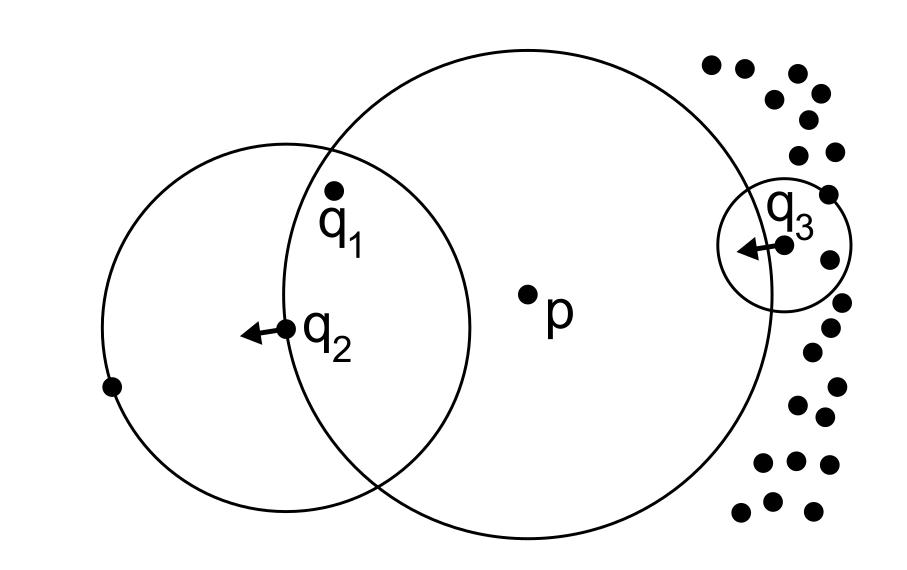
\includegraphics[width=\textwidth]
    {imagenes/aleatoria.jpeg}}
    \caption{\label{fig:aleatoria} Ejemplo de situación para proyección aleatoria}
\end{figure}

Después de la proyección, $p$ tendría $q_3$ como vecino en lugar de $q_2$, 
lo que resultaría en un aumento sustancial en la densidad relativa 
asociada con ese vecino. Si muchos vecinos son reemplazados de esta 
manera tendríamos un cambio considerable en los resultados finales.

Como alternativa a la estimación de $LOF(p)$ por $LOF(p')$, en su
lugar se propone que el cálculo de $LOF(p)$ se calcule en él, 
espacio original, pero se calcule utilizando el vecindario 
y distancias de vecindario según lo determinado después de la 
proyección.


La idea por tanto será, en lugar de pagar el alto costo del cálculo 
del k-vecino más cercano en el espacio original, podemos determinar 
un vecindario más grande dentro del espacio de proyección e 
invertir el mapeo para obtener estimaciones de los vecinos en el 
espacio original. Si se considera un número suficiente de vecinos 
en el espacio de proyección (donde el número depende de la dimensión 
intrínseca de $D'$), el verdadero conjunto original de k-vecinos se 
puede recuperar con muy alta probabilidad. Esto nos supondría una 
alta reducción de coste computacional. Veamos las etapas en la siguiente
figura que nos proporciona el artículo de referencia \cite{vriesFindingLocalAnomalies2010}


\begin{figure}[H]
    \center{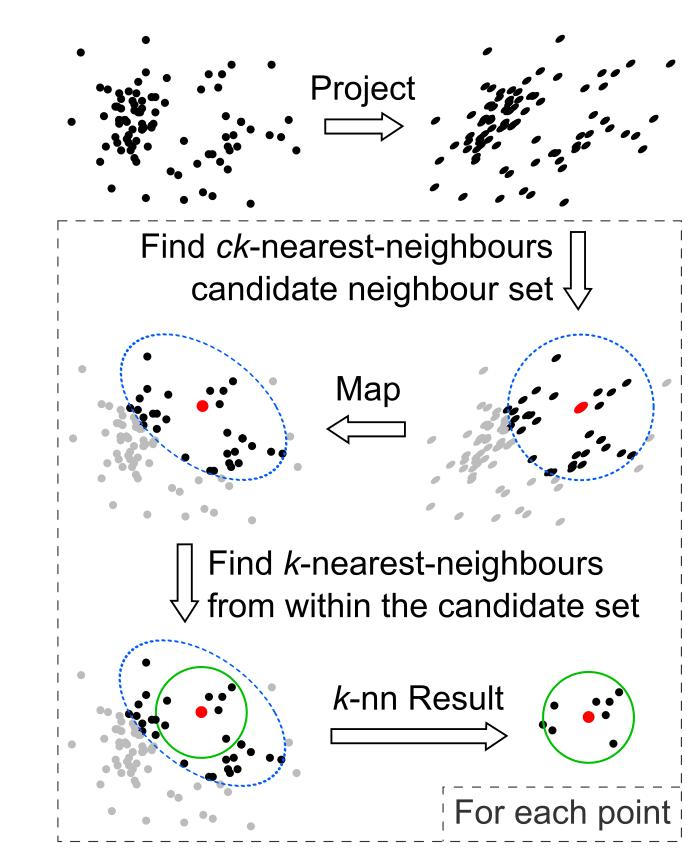
\includegraphics[width=\textwidth]
    {imagenes/etapas-pinn.jpeg}}
    \caption{\label{fig:pinn} Etapas del algoritmo PINN}
\end{figure}

Con estos resultados y teniendo calculado el conjunto de los k-vecinos
más cercanos, en nuestro caso usaremos $LOF$ para el cálculo final de
las puntuaciones.

Vamos a exponer el pseudocódigo del algoritmo para entender mejor su funcionamiento:

\begin{codigo}
    \begin{algorithmic}[1]
    \Function {RP+PINN+LOF}{Matrix de datos D,k,t,s,h }
    \State \parbox[t]{305pt}{\textbf{RP:} Realizamos una projección aleatoria $D \rightarrow Y$}
    \State \textbf{PINN}: h define el tamaño del set de candidatos.
    
    \ForEach{$p \in \mathcal D $}
    \State \parbox[t]{305pt}{ 1) encontrar los h-vecinos más cercanos en el espacio $y$}
    \State {2) Mapeamos el vecindario calculado con los puntos en el espacio original $D$}
    \State {3) Calculamos los k-nn vecinos más cercanos para $p$ dentro del vecindario}   
    \EndFor
    \State \textbf{LOF}: Aplicamos $LOF$.
    \State \Return Puntuaciones: $LOF$
    \EndFunction 
    \end{algorithmic}
\end{codigo}


Como podemos ver, a pesar de que intrínsecamente estamos usando $LOF$ como
sistema de puntuación de anomalías, la idea es crear un proceso para permitir
su aplicación en dimensiones superiores sin caer en la maldición de la
dimensionalidad. De este modo tenemos un proceso efectivo y rápido. En 
nuestro caso al realizar una implementación en Python hemos aprovechado 
al máximo las herramientas de este lenguaje para buscar la máxima eficiencia.

\section{OUTRES}
Para el desarrollo de este algoritmo hemos usado como referencia el
artículo donde se desarrolla con máximo detalle \cite{mullerAdaptiveOutliernessSubspace2010}

Esta técnica nace a partir de una idea clara, en las técnicas tradicionales
se establecen las anomalías a través del uso de todo el espacio. Pero de ese
modo nos estamos perdiendo lo que hay escondido en las proyecciones de subespacios.
Por tanto, la propuesta es desarrollar una puntuación de anomalías basada 
en la desviación de objetos en las proyecciones subespaciales. Principalmente
se centra en obtener la puntuación midiendo su grado de desviación local.
Además, solo se hará uso de un subconjunto de atributos y no del espacio
completo, y es que un objeto puede mostrar una alta desviación en 
comparación con su vecindario en un subespacio. Además, el mismo 
objeto puede agruparse con otros objetos en un segundo subespacio y 
puede no aparecer como un valor atípico. O por otro lado aparecer en 
un tercer subespacio disperso donde todos los objetos parecen ser 
valores atípicos. Veamos un ejemplo de esto en la siguiente figura:


\begin{figure}[h]
    \center{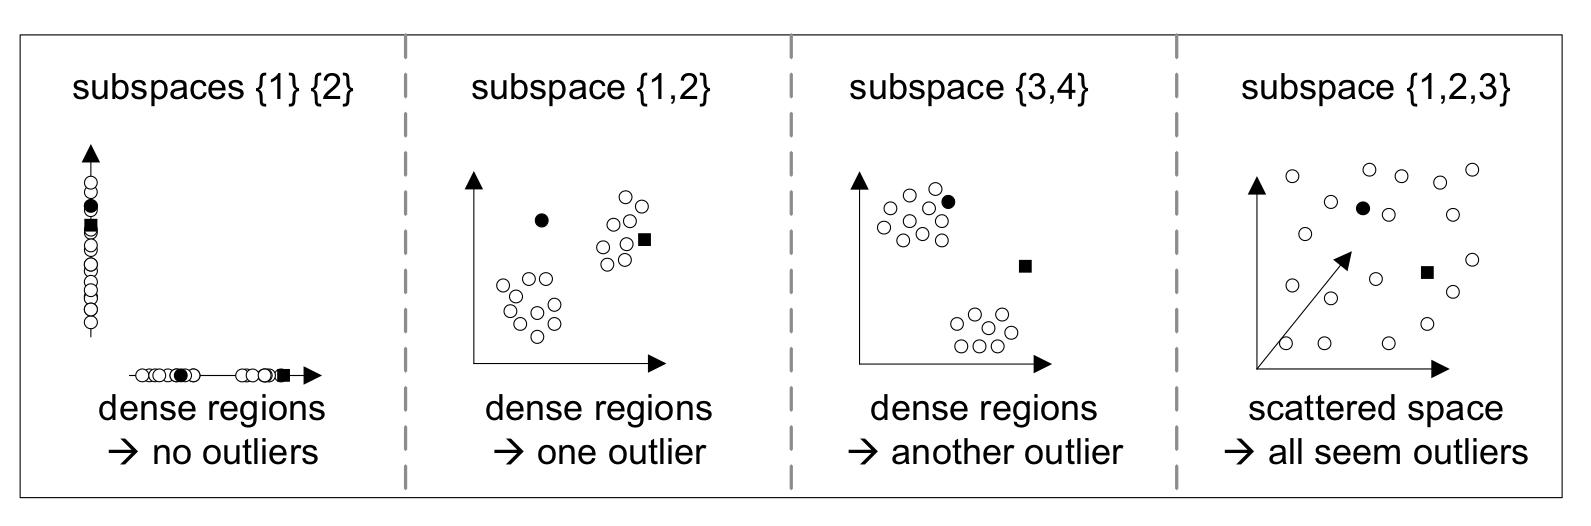
\includegraphics[width=\textwidth]
    {imagenes/subespacios.jpeg}}
    \caption{\label{fig:subespacios} Anomalías en diferentes subespacios}
\end{figure}

Como podemos ver es posible que cada anomalía necesite una proyección para
poder detectarla de forma clara. Las técnicas de reducción de dimensionalidad 
global, como el análisis de componentes principales PCA, proporcionan 
una única proyección para todos los objetos. En contraste, nuestro objetivo es 
detectar múltiples subespacios relevantes por objeto. La agrupación en subespacio 
detecta múltiples proyecciones, sin embargo, se centra en subespacios para grupos 
de objetos agrupados. Para la clasificación de valores atípicos, el enfoque está 
en los objetos y subespacios individuales en los que un valor atípico se desvía 
mucho de su vecindario local. Un enfoque muy novedoso.


El método se basa en dos pilares principalmente. Primero, para cada objeto, 
seleccionamos estadísticamente un conjunto de proyecciones para la puntuación 
de valores atípicos. En estas proyecciones interesantes, existe la posibilidad
de encontrar valores atípicos o aumentar su puntuación. Por otro lado, los subespacios
se distribuyen de forma uniforme por lo que no aportan información y pueden ser
ignorados. En segundo lugar, la desviación del objeto aumenta con el número de
atributos en un subespacio relevante. Las distancias entre objetos crecen cada vez
más con la maldición de la dimensionalidad. Por tanto, cuando crece la dimensionalidad
los puntos suelen a estar más dispersos.


El algoritmo que se propone basado en todos estos conceptos es OUTRES donde solo se
usaran una selección de proyecciones no distribuidas uniformemente. Además, ya que el
calculo de desviación se realiza en varios subespacios con diferente dimensión, se propone
un método adaptativo con el número de atributos para el cálculo del score en cada subespacio.

Para describir el procedimiento del algoritmo seguiremos la notación de \cite{mullerAdaptiveOutliernessSubspace2010}
para facilitar su complementación con el artículo. La primera idea que debemos de desarrollar es
la de cómo combinar los resultados de diferentes subespacios para un mismo punto.
Para ello se usa la expresión
\[ r(o) = \prod_{S \in RS(o)} score(o,S)  \]

Donde el conjunto $Rs(o)$ representa el conjunto de subespacios relevantes para el objeto
$O$. Como podemos ver se calcula una agregación de los resultados de cada subespacio.

A continuación, debemos de resolver la incógnita de como seleccionar los subespacios
relevantes para cada objeto $o$. En primer lugar, para determinar si es interesante se
realizara un test estadístico para comprobar si esta uniformemente distribuido. Si 
solo aplicamos esto, deberíamos de realizar dicho test a todos los subespacios posibles.
Pero para evitar esto definimos un subespacio como uniformemente distribuido si todos sus
componentes también son uniformemente distribuidos. Así descartamos un subespacio
tan pronto como al menos un atributo este uniformemente distribuido. Con esta técnica
podemos realizar una alta poda en el momento en el que detectamos un atributo uniforme.
Veamos cómo funciona en la siguiente figura: 

\begin{figure}[h]
    \center{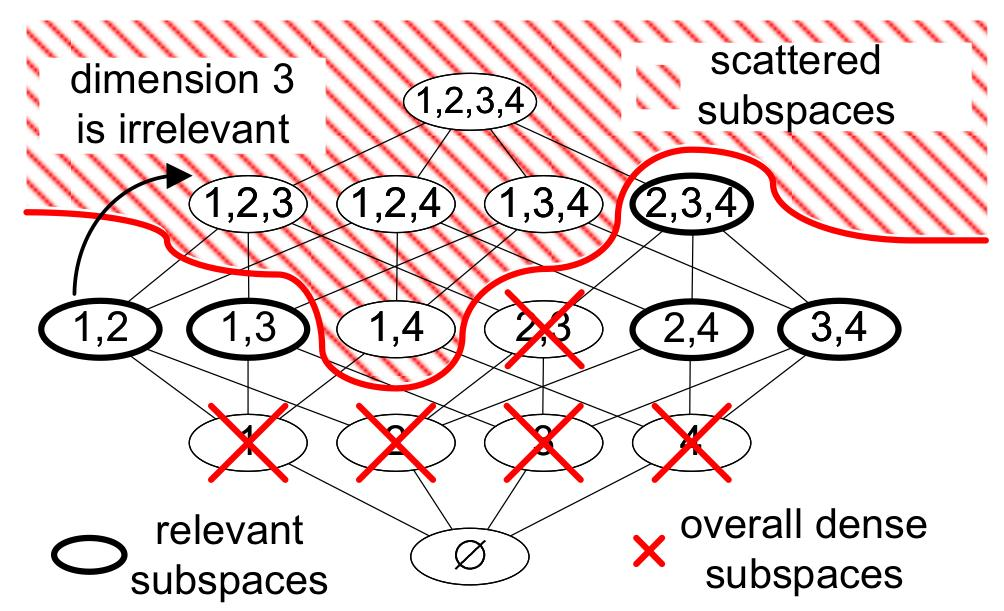
\includegraphics[width=\textwidth]
    {imagenes/seleccion-subespacios.jpeg}}
    \caption{\label{fig:select-subespacios} Selección de subespacios}
\end{figure}

En este caso conseguiríamos un gran coste computacional y no tendríamos que realizar los
test estadísticos ni ningún calculo más para aquellos subespacios que no aportan información.

Ahora vamos a explicar cómo se implementa el cálculo adaptativo de score para cada subespacio.
La idea es poder realizar un cálculo que permita su agregación independientemente de la 
dimensión del subespacio donde se está calculando.

Lo primero es plantear un vecindario adaptativo:

\[ AN(o,S) = \lbrack p | dist_S(o,p)= <= \epsilon(|S|) \rbrack  \]

La idea general es derivar el rango variable de una observación común en 
las proyecciones del subespacio. Mientras aumenta el número de atributos 
en una proyección subespacial, el volumen de un vecindario fijo disminuye 
significativamente en comparación con el volumen general del subespacio.

Ahora necesitamos una técnica para calcular la densidad en el vecindario,
que definimos como 

\[ den(o,S) = \frac{1}{|DB|} \sum_{p \in DB} K_e ( \frac{dist_S(o,p)}{h} ) \]

Donde $k_e$ es una función kernel en nuestro caso el kernel de Epanechnikov
que se define como

\[ K_e(x) = (1-X^2), x < 1\]

y definimos h como el parámetro de ancho de banda que se usa para escalar 
la influencia de cada objeto a una distancia máxima de h. Existe una expresión
para calcular el h optimo la cual se ha implementado y tiene en cuenta el volumen
de la dimensión como comentábamos antes que era importante.

Con esta h optima ya que se tiene en cuenta el volumen del subespacio como comentábamos
en la definición del vecindario adaptativo, podemos usarlo para el cálculo del tamaño
de dicho vecindario:


\[ \epsilon(|S|) = \epsilon \cdot \frac{h_{optimal}(|S|)}{h{optimal}(2)} \]


Por lo tanto, simplemente escalamos el ancho de banda inicial dado del espacio 2d 
al espacio de datos completo y utilizamos estos valores para la estimación de 
densidad. Ahora solo necesitamos calcular la desviación de la densidad.

\[dev(o,S) = \frac{\mu - den(o,S)}{2 \cdot \sigma} \]

Donde $\mu$ representa la media de la densidad y $\sigma$ la desviación estándar.

A pesar de que exista desviación solo la usaremos como score si dicha desviación es
significativa. De modo que ya tenemos todas las herramientas para definir nuestra función
de puntuación como:

\[ score(o,S) = \left\{ \begin{array}{lcc}
    \frac{den(o,S)}{dev(o,S)} si  dev(o,s) >=1 \\
    \\ 0 
    \end{array}
\right.\]

Como podemos ver es un proceso complejo el de selección de subespacios y análisis de 
cada subespacio. Como veíamos que los subespacios se componían de forma combinatoria,
una buena forma para implementar este algoritmo será con un enfoque recursivo. Aquí podemos
ver una descripción de OUTRES:



\begin{codigo}
    \begin{algorithmic}[1]
    \Function {OUTRES}{o,S }    
    \ForEach{$i \in \mathcal D \setminus S $}
    \State \parbox[t]{305pt}{$ S' = S \cup \lbrace i \rbrace $}
    
    \If{$S'$ es relevante( realizar test estadistico)}
    \State $den(o,S') = \frac{1}{|DB|} \sum_{p \in DB} K_e ( \frac{dist_{S'}(o,p)}{h}$
    \State $dev(o,S') = \frac{\mu - den(o,S')}{2 \cdot \sigma}$
    \If{$dev(o,S') >= 1$ alta desviación}
    \State $r(o) = r(o) \cdot \frac{den(o,S)}{dev(o,S)} $  agregar score
    \EndIf
    \State \textbf{OUTRES}(o,S')
    \EndIf  
    \EndFor
    \EndFunction 
    \end{algorithmic}
\end{codigo}

Este algoritmo como podemos ver en planteamiento es muy interesante ya que usa la 
recursividad de llamadas para conseguir la combinatoria entre subespacios de forma
fácil. El problema que 
plantea es su complejidad que es de $O(2^n \cdot n^2)$ debido a la combinatoria entre
todos los posibles subespacios. Como sabemos este es el peor de los casos y si se consigue
que haya poda, la eficiencia será mucho mejor. Veremos en la práctica más adelante como
afronta esta complejidad dicho algoritmo.


\section{ODIN}
Se ha desarrollado el algoritmo ODIN, el cual se presenta en \cite{hautamakiOutlierDetectionUsing2004}. 
\textbf{Outlier Detection using Indegree Number (ODIN)} es un algoritmo que hace uso 
del grafico de los k-vecinos más cercanos. Por tanto, el objetivo será desarrollar un 
algoritmo que a partir del algoritmo de k-vecinos más cercano se realice una mejora que 
nos ofrezca un mejor desempeño.

Se propone un algoritmo para calcular las anomalías, como idea base partimos del  
grafo de k-vecinos más cercanos. En este grafo cada nodo es un vector de datos o  
un ejemplo de datos. Los bordes de conexión entre dos vértices $v_i$ y $v_j$ se produce 
si $v_j$ esta entre los k-vecinos más cercanos de $v_i$. Este razonamiento se aplica a todos 
los vértices y obtenemos el grafo knn. Con dicha definición el grafo es dirigido ya que 
podemos tener conexiones en un sentido, pero no en el contrario. Pensemos en el ejemplo de una 
anomalía y un punto en una región densa. Podemos tener conexión de la anomalía al punto pero  
muy probablemente no tengamos la conexión reciproca. Además, el grafo tendrá pesos para 
cada conexión, determinando la distancia entre los diferentes puntos. Como tenemos en cuenta 
los k-vecinos más cercanos sabemos a priori que cada vértice tendrá k conexiones. Para la construcción 
de este grafo será necesario el cálculo de todas las distancias entre puntos y por tanto, 
una complejidad de $O(n^2)$.

En nuestro caso, \textbf{ODIN} hace uso del concepto de k-vecinos más cercanos mutuos (MkNN).
Para ello se define que dos vértices serán vecinos mutuos si en el grafo knn existen  
las conexiones entre $v_i$ y $v_j$, y reciproca $v_j$ y $v_i$. Deben existir ambas para que 
exista conexión. De modo que este grafo es no dirigido y podemos seguir teniendo pesos con la 
distancia entre ambos vectores.

Con el uso del grafo de k-vecinos más cercanos mutuos tenemos una definición muy intuitiva de que
es una anomalía. Para explicar el razonamiento y ver un ejemplo más claro, podemos usar
un ejemplo ya visto con anterioridad.


\begin{figure}[h]
    \center{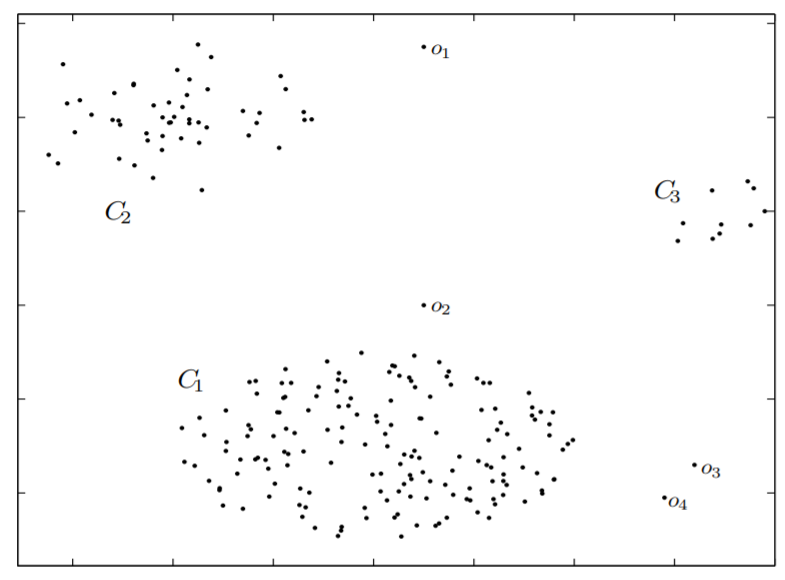
\includegraphics[width=\textwidth]
    {imagenes/datos-dispersos.png}}
    \caption{\label{fig:explica-knn} Ejemplo de anomalías}
\end{figure}


En este caso como podemos ver al generar los vecinos mutuos $O_1$ se quedaría sin vecinos 
ya que el resto de puntos de $C_2$ no lo considerarían como vecino mutuo. Por tanto, ya tenemos 
una definición intuitiva de outlier. Por un lado, los vértices con conexiones formarán 
clústeres mientras que los vértices sin conexiones serán las anomalías. 

En este ejemplo también podemos ver el problema que plantea esta definición. Pensemos en el  
punto $O_2$, es decir, un punto más cercano al clúster pero que es una anomalía. 
Puede entrar lo posibilidad de que algunos puntos del borde del clúster consideren al  
punto $O_2$ como un vecino mutuo y de este modo ya podría ser clasificado como un punto 
normal. Es necesario introducir cierta flexibilidad. Para ello en lugar de usar si tiene o no  
conexiones se usa el grado del vértice y se compara con un parámetro de entrada $T$ que funciona 
de umbral y podemos ajustar para ser más o menos restrictivos.

Ya tenemos los conceptos y la idea que sigue el algoritmo para detectar anomalías.
Vamos a plantear el procedimiento:


\begin{codigo}
    \begin{algorithmic}[1]
    \Function {ODIN}{S,k,T }  
    \State Calcular el grafo Mknn de S  
    \For{$i =1$ to $|S| $}
    \If{Grado de $v_i \leq T$ }
    \State \parbox[t]{305pt}{Marcar $v_i$ como anomalía}
    \EndIf  
    \EndFor
    \EndFunction 
    \end{algorithmic}
\end{codigo}


Como podemos ver el procedimiento es simple, primero calculamos el grafo
de vecinos mutuos y después con el grado de cada vértice determinamos si es
una anomalía si supera o no el umbral establecido por parámetro. 

  
Como podemos ver en este caso no realizamos el cálculo de ningún score si no que
se calcula una etiqueta binaria $0-1$ si es anomalía o no. Este tipo de resultado
ya lo explicamos anteriormente y aunque podríamos generar un score usando como
puntuación el grado de cada punto. En este caso hemos considerado interesante,
para ampliar la variedad de nuestra biblioteca, mantener la salida de etiqueta
binaria. De modo que mantenemos el enfoque de los autores.

  
Por otro lado, debemos mencionar que el parámetro $T$ puede plantear dificultades
para ajustarlo ya que realmente debemos de encontrar el umbral correcto y
será determinante para los resultados.


\section{MeanDIST y KDIST}
Vamos a tratar estos dos algoritmos en la misma sección ya que ambos se basan en
los mismos conceptos y se diferencian en el cálculo final. Los dos algoritmos parten 
de la idea expuesta en \cite{ramaswamyEfficientAlgorithmsMining2000} que se plasma 
en el algoritmo \textbf{RSS}.

Los conceptos que se plantean en \textbf{RSS} son muy básicos y fácil de comprender.
El algoritmo lo que hace es calcular los k-vecinos más cercanos y considerar anomalías
los $n$ puntos con las distancias a su k-vecino más grande. La idea es ordenar los puntos
por su distancia mayor en su vecindario y aquellos con distancias más grandes son aquellos
que no están en un clúster y, por tanto, anomalías. Como podemos ver el razonamiento es
fácil de comprender, pero presenta multitud de inconvenientes. En primer lugar, la definición
de anomalía puede no ser suficiente en multitud de casos, pero el principal problema 
es estimar $n$. Estamos suponiendo que a priori conocemos el número exacto de anomalías
que debemos detectar en los datos. Esto en la práctica no tiene funcionalidad.

A partir de esta idea y como mejora a los problemas que plantea, nacen los dos algoritmos
que analizamos en esta sección. En primer lugar el algoritmo \textbf{MeanDIST} usa
la media de las distancias en su vecindario para ordenar a los vértices. \textbf{KDIST} 
usará el máximo de las distancias a sus k-vecinos más cercanos. Hasta este punto no  
tenemos una mejora clara, pero la clave y la mejora reside en introducir un umbral como 
hacíamos en \textbf{ODIN} que sea más flexible y que además en este caso se calcule  
de forma inteligente.

Cuando analizamos la lista ordenada de distancias de menor a mayor, podemos comprobar
si la diferencia entre las distancias adyacentes es mayor que un determinado umbral $T$.
Para definir este umbral o punto de corte T usamos la siguiente ecuación

\[ T = max(L_i - L_{i-1}) * t \]

donde $L_i$ puede ser o la distancia calculada con \textbf{KDIST} o \textbf{MeanDIST}
del elemento i-ésimo. por otro lado $t$ será un valor entre $[0-1]$ que el usuario define 
por parámetro.

Para entender el cálculo del umbral veamos la siguiente figura que nos muestra la diferencia
entre los vectores ordenados.


\begin{figure}[h]
    \center{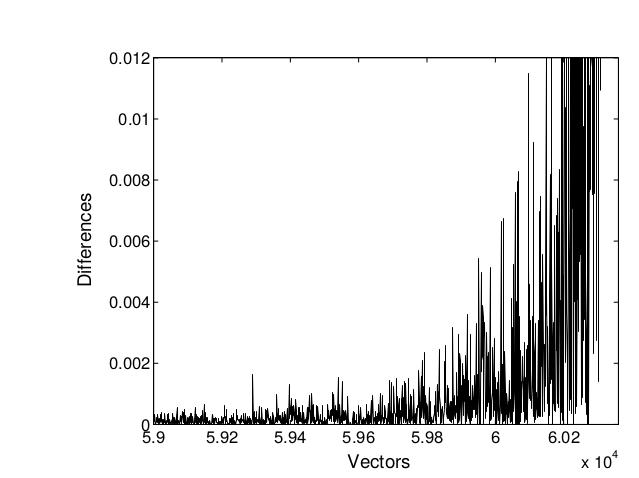
\includegraphics[width=\textwidth]
    {imagenes/salto-diferencia.jpeg}}
    \caption{\label{fig:explica-salto} Diferencia entre vectores ordenados por distancia}
\end{figure}


Como podemos ver existe un punto donde se produce un salto en la diferencia entre los vectores
ordenados. Aquí reside la definición de anomalía de estos dos algoritmos ya que podemos entender
que cuando se produce dicho salto estamos hablando de anomalías, vectores que se encuentran
muy distanciados del resto de datos. 

De modo que en el cálculo de este umbral estamos calculando en primer lugar la diferencia
más pronunciada que se produce en nuestros datos. Después establecer la amplitud de este
umbral y la permisión que admitimos con el parámetro $t$ definido por el usuario. 

Por tanto, con el cálculo del punto de corte entre los datos 
normales y las anomalías. Con estos conceptos definimos los algoritmos de la siguiente forma

\begin{codigo}
    \begin{algorithmic}[1]
    \Function {MeanDIST y KDIST}{S,k,t }  
    \State Calcular T
    \State Calcular el grafo knn de S
    \State L = vector ordenado ascendentemente
    \State Encontrar el i mas pequeño para el cual $ l_i - L_{i-1}  \geq T$
    \State Marcar como anomalia $L_i , ... , L_{|S|}$ 
    \EndFunction 
    \end{algorithmic}
\end{codigo}

La complejidad del algoritmo está marcada por el cálculo del grafo knn que conlleva
el cálculo de todas las distancias, es decir $O(n^2)$.